\chapter{\IfLanguageName{dutch}{Stand van zaken}{State of the art}}%
\label{ch:stand-van-zaken}

% Tip: Begin elk hoofdstuk met een paragraaf inleiding die beschrijft hoe
% dit hoofdstuk past binnen het geheel van de bachelorproef. Geef in het
% bijzonder aan wat de link is met het vorige en volgende hoofdstuk.

% Pas na deze inleidende paragraaf komt de eerste sectiehoofding.

Bedrijven slaan veel data op. Doordat deze data nuttig kan zijn voor het identificeren van nieuwe kansen is het belangrijk om deze data klaar te maken voor business analytics. Dit is het proces van verzamelen, organiseren, analyseren en interpreteren van gegevens om inzichten te krijgen. Er kan bijvoorbeeld gekeken worden naar klantgegevens om zo patronen en trends te vinden in het gedrag van de klant~\autocite{PratibhaKumari2023}.

Doordat bedrijven vaak werken met veel verschillende soorten data dat op verschillende plekken opgeslaan wordt, is het vaak belangrijk dat deze data eerst opgekuist, getransformeerd en georganiseerd moet worden. Dit is waarbij het implementeren van ETL's en ELT's van pas komt~\autocite{Inmon2023}.

\section{Wat zijn ETL's of ELT's?}

ETL's en ELT's zijn processen die organisaties gebruiken voor het verzamelen en samenvoegen van data uit meerdere bronnen. Bij ETL's wordt de data getransformeerd voor het naar de doelopslagplaats geladen wordt, terwijl dit bij ELT's pas achteraf gebeurd. Daardoor staat ETL voor Extract, Transform and Load en ELT voor Extract, Load and Transform~\autocite{Bartley2023}.

Verder in de bachelorproef zal er alleen gesproken worden over ETL's. Dit doordat de beste manier om een ETL te implementeren wordt onderzocht.

\section{Welke soorten ETL tools bestaan er?}

Er bestaan verschillende soorten ETL tools. Zo zijn er de cloud-based ETL tools. Deze worden gehost op cloud infrastructure, zijn zeer schaalbaar en bieden pay-as-you-go prijs modellen aan~\autocite{Ethan2024}.

Daarnaast zijn er ook on-premises ETL tools. Deze worden gehost op de infrastructuur van het bedrijf waardoor het bedrijf er de volledige controle over heeft~\autocite{Ethan2024}.

Afhankelijk van wat men nodig heeft kan er ook gekozen worden voor hybrid ETL tools. Dit is een combinatie van het gebruik van cloud-based tools met het gebruik van on-premises tools~\autocite{Ethan2024}.

Ten slotte zijn er ook open source ETL tools. Dit zijn gratis ETL tools. Voorbeelden hiervan zijn Portable, Apache NiFi, AWS Glue, Airbyte en Informatica~\autocite{Ethan2024}.

\section{Populairste cloud-based ETL tools}

Zoals te zien in de enquête van~\textcite{vines2023overview} is Microsoft Azure, gevolgd door Amazon Web Services (AWS) en Google Cloud Services, de populairste cloud provider. Deze cloud-providers bieden dan ook de meest populaire cloud-based ETL tools aan. 

Microsoft biedt bijvoorbeeld Azure Data Factory, Azure Databricks, Azure Synapse Analytics en Microsoft Fabric aan. Hier wordt later verder op in gegaan in de literatuurstudie.

%Binnen Azure Data Factory kan er gebruik gemaakt worden van Mapping Data Flows, dit is een code-vrije manier waarmee ETL's opgebouwd kunnen worden. De logica achter de ETL kan hierna makkelijk getest worden op live data en samples~\autocite{Kromer2022}.

Ook Amazon Web Services (AWS) en Google Cloud Services bieden ETL tools aan. Zo heeft AWS bijvoorbeeld AWS Glue~\autocite{Khan2024} en Google Cloud heeft Google Data Fusion~\autocite{Jaiswal2022}.

\section{Infrastructure as Code (IaC)}

Infrastructure as Code (IaC) is een belangrijk concept in de wereld van moderne softwareontwikkeling. Doordat dit door Net IT gebruikt wordt, zal het ook gebruikt worden als vergelijkingscriteria voor de proof-of-concepts. Het is dus belangrijk om te begrijpen wat het is.\\ 

IaC stelt teams in staat om infrastructuur te beheren met behulp van definitiebestanden, in plaats van fysieke hardwareconfiguratie of interactieve configuratietools. Deze bestanden helpen bij het automatiseren van het opzetten en onderhouden van infrastructuur, wat resulteert in snellere ontwikkelcycli en hogere betrouwbaarheid. Dit betekent dat de gehele infrastructuur, inclusief netwerken, virtuele machines en verbindingen, kan worden beheerd met scripts of declaraties. Het voordeel hiervan is dat er voor zowel de development en productie environment dezelfde infrastructuur opgezet kan worden. Het is dus snel en consistent. Doordat de definitiebestanden in IaC in source control opgeslaan kunnen worden, kunnen ook zo fouten makkelijker opgespoord worden~\autocite{Schults2024}.

\section{Continuous Integration (CI) en Continuous Deployment (CD)}

Bij Continuous Integration (CI) wordt de code van één of meerdere developers samen gevoegd, getest en gebouwd. Dit gebeurd continu. Een voorbeeld hiervan is dat een developer de code van zijn/haar GitHub branch merged op de ``main'' (of ``master'') branch van het project. Het doel van CI is dat deze ``main'' (of ``master'') branch gezond blijft en dat nieuwe aanpassingen door meerdere developers niet zorgt voor fouten in de code die resulteren in het falen van een build~\autocite{Jackson2020}.\\

Continuous Delivery (CD) is een uitbereiding van Continuous Integration. Het is het automatiseren van het release process. Het zorgt er voor dat aanpassingen frequent gedeployed kunnen worden~\autocite{Jackson2020}.\\

Ten slotte is er ook Continuous Deployment. Dit is een uitbereiding op Continuous Delivery en zorgt er voor dat code changes automatisch naar productie worden gepusht~\autocite{Jackson2020}.\\

Continuous Integration (CI) en Continuous Deployment (CD) kan ook gebruikt worden in combinatie met Infrastructure as Code (IaC) om zo wijzigingen aan de infrastructuur van een project te automatiseren.

\section{Microsoft Azure}

Microsoft Azure is een cloud computing-platform die door Microsoft wordt aangeboden. Het biedt een breed scala aan cloudgebaseerde oplossingen en services waarmee bedrijven en ontwikkelaars applicaties kunnen bouwen, implementeren en beheren. \\

\begin{figure}[H]
    \centering
    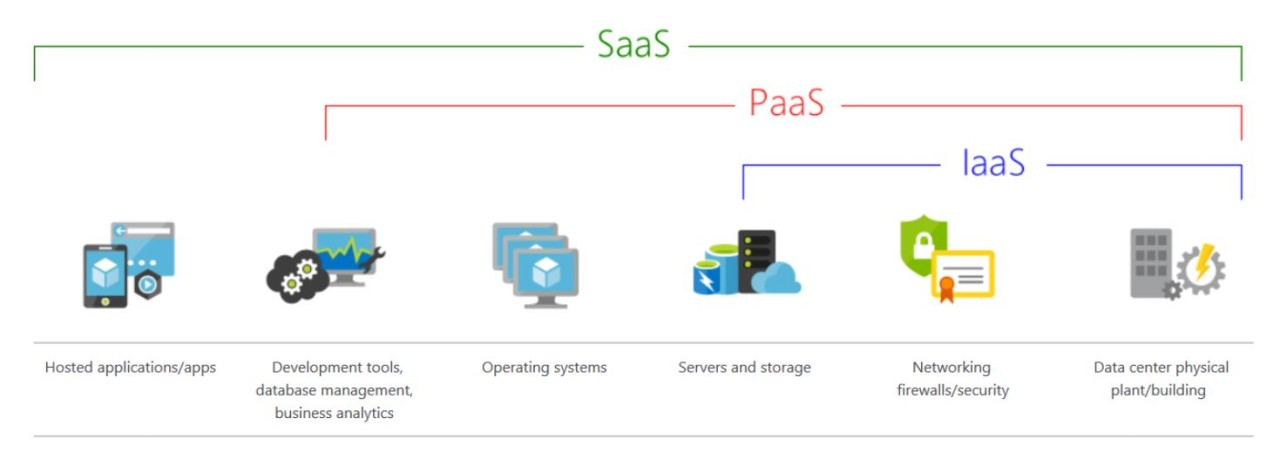
\includegraphics[width=1\textwidth]{./graphics/standvanzaken/verschillen.jpg}
    \caption{Verschillen tussen IaaS, PaaS en SaaS~\autocite{Stoenescu2021}}
\end{figure}

Met Azure kunnen bedrijven gebruikmaken van Infrastructure as a Service (IaaS), waardoor ze onder andere virtuele machines, opslag en netwerken kunnen huren op basis van hun behoeften. Dit geeft organisaties de flexibiliteit om snel op te schalen zonder dat ze fysieke servers hoeven aan te schaffen. Daarnaast biedt het platform ook een Platform as a Service (PaaS), waarmee ontwikkelaars zich kunnen concentreren op het ontwikkelen van applicaties zonder zich zorgen te hoeven maken over de onderliggende infrastructuur. Ten slotte is er ook Software as a Service. Hierbij wordt er een applicatie gehost en beschikbaar gemaakt voor de gebruiker op basis van een subscription. Voorbeelden hier van zijn bijvorbeeld officetools (Microsoft Office 365)~\autocite{Suneetha2024}. \\

Azure is sterk in dataopslag en -beheer, waarbij veilige en schaalbare opties worden aangeboden voor zowel gestructureerde als ongestructureerde gegevens. Bovendien kunnen organisaties gebruikmaken van analyse- en big data-services zoals Azure Synapse Analytics en HDInsight om inzichten te verkrijgen die strategische beslissingen ondersteunen~\autocite{Awati2023}. \\

Darnaast biedt Azure ook encryptie, toegangsbeheer en compliance-certificeringen om gegevens veilig te houden~\autocite{Siddiqui2023}.

\subsection{ETL Services}

Volgende Azure Services zijn services die gebruikt kunnen worden voor het implementeren van ETL's of ELT's.

\subsubsection{Azure Data Factory (ADF)}

Azure Data Factory is een Platform as a Service (PaaS) voor het implementeren van ETL's en ELT's. Zowel on-premises als cloudgegevensbronnen worden hierbij ge ondersteund voor het verplaatsen van gegevens~\autocite{Rawat2019}.\\

%\textbf{Onderdelen}

Azure Data Factory is opgebouwd uit verschillende onderdelen. Als eerste hebben we een pipeline. Dit is een groep van activiteiten die een reeks processen uitvoert zoals bijvoorbeeld het extraheren of transformeren van gegevens. Een voorbeeld van een activity is een Mapping Data Flow. Hiermee kan men logica voor datatransformaties ontwikkelen zonder code te schrijven. Daarnaast zijn er ook datasets. Dit is een representatie of verwijzing naar de daadwerkelijke gegevens in gegevensopslag. Een dataset is steeds gekoppeld aan een linked service. Deze slaan de informatie op die Azure Data Factory nodig heeft voor het connecteren naar een externe dataopslag. Een pipeline wordt uitgevoerd door een trigger. Er zijn veel verschillende soorten triggers voor veel verschillende soorten events. Daarnaast kan er voor een pipeline parameters gedefinieerd worden. Dit zijn read-only key-value pairs die een configuratie vormen. Ook kunnen er variables gebruikt worden om tijdelijk waardes op te slaan. In combinatie met parameters kunnen dan waardes tussen pipelines, data flows, en andere activities door gegeven worden. Wanneer een pipeline wordt uitgevoerd zal er een pipeline run aangemaakt worden~\autocite{Microsoft2024a}.\\

%\textbf{Mapping Data Flows}

Met behulp van Mapping Data Flows kunnen ETL's geïmplementeerd worden zonder hiervoor gebruik te moeten maken van code~\autocite{Kromer2022}. De resulterende data flows worden uitgevoerd als activities binnen een Azure Data Factory pipeline dat gebruik maakt van Apache Spark Clusters. Deze Mapping Data Flows maken gebruik van data flow scripts. Dit zijn artifacten die gegenereerd worden door de UI. Het is een taal die de data transformatie beschrijft dat de Spark Cluster zal moeten uitvoeren. De UI van Azure Data Factory beheert het data flow script maar het script kan ook bekeken en handmatig bewerkt worden~\autocite{Kromer2022a}.

In Mapping Data Flows kunnen verschillende soorten transformaties gedaan worden zoals bijvoorbeeld het joinen, het filteren of selecteren van data.

%\begin{itemize}
%    \item Multiple inputs/outputs
%    \begin{itemize}
    %        \item New Branch
    %        \item Join
    %        \item Conditional Split
    %        \item Exists
    %        \item Union
    %        \item Lookup
    %    \end{itemize}
%    \item Schema modifier
%    \begin{itemize}
    %        \item Derived Column
    %        \item Select
    %        \item Aggregate
    %        \item Surrogate Key
    %        \item Pivot
    %        \item Unpivot
    %        \item Window
    %        \item Rank
    %        \item External Call
    %    \end{itemize}
%    \item Formatters
%    \begin{itemize}
    %        \item Flatten
    %        \item Parse
    %        \item Stringify
    %    \end{itemize}
%    \item Row modifier
%    \begin{itemize}
    %        \item Filter
    %        \item Sort
    %        \item Alter Row
    %        \item Assert
    %    \end{itemize}
%    \item Flowlets
%    \begin{itemize}
    %        \item Flowlet
    %    \end{itemize}
%    \item Destination
%    \begin{itemize}
    %        \item Sink
    %    \end{itemize}
%\end{itemize}

%\subsubsection{Pipeline}
%
%Een pipeline een groep van activiteiten die een reeks processen uitvoert zoals bijvoorbeeld het extraheren of transformeren van gegevens.
%
%\subsubsection{Datasets}
%
%Een dataset is een representatie of verwijzing naar de daadwerkelijke gegevens in gegevensopslag.
%
%\subsubsection{Linked Services}
%
%Linked Services slaan de informatie op die Azure Data Factory nodig heeft voor het connecteren naar een externe data-opslag.
%
%\subsubsection{Activity}
%
%Activities representeren een processing step binnen een pipeline. 
%
%\subsubsection{Mapping Data Flows}
%
%Met datastromen kunnen men logica voor datatransformaties ontwikkelen zonder code te schrijven. De resulterende data flows worden uitgevoerd als activities binnen Azure Data Factory pipelines.
%
%\subsubsection{Integration Runtime}
%
%Een integration runtime vormt de brug tussen de activity en de gekoppelde service. 
%
%\subsubsection{Triggers}
%
%Triggers beslissen wanneer een pipeline uitgevoerd moet worden. Er zijn verschillende soorten triggers voor verschillende soorten events. 
%
%\subsubsection{Pipeline runs}
%
%Een pipeline run is een instance van een pipeline execution. 
%
%\subsubsection{Parameters}
%
%Parameters zijn read-only key-value pairs die een configuratie vormen. 
%
%\subsubsection{Control flow}
%
%\subsubsection{Variables}
%
%Variables kunnen gebruikt worden in een pipeline om tijdelijk waardes op te slaan. Het kan ook gebruikt worden in combinatie met parameters om waardes tussen pipelines, data flows en andere activities door te geven.
%
%Azure IR
%
%Self-Hosted IR

\subsubsection{Azure Databricks}

Azure Databricks is een geavanceerd platform voor data-analyse dat zich integreert met Azure services. Het biedt een complete omgeving voor het ontwikkelen, implementeren en delen van krachtige data-analyses en AI-toepassingen op grote schaal. Het integreert zich ook met de opensource-community zoals bijvoorbeeld Delta Lake, Delta Sharing, MLflow, Apache Spark en Redash. Veel voorkomende use cases van Azure Databricks zijn het bouwen van een data lakehouse voor ondernemingen, het implementeren van ETL's, gebruik van machine learning en dergelijke~\autocite{Microsoft2024}.

Het verschil met Azure Data Factory is dat de ETL’s worden geïmplementeerd via code en niet via UI tools. Azure Databricks is gebaseerd op het Apache Spark opensource project. Het grote voordeel is dat het platform het toelaat om makkelijker te kunnen samen werken. Daarnaast is Apache Spark niet enkel gelimiteerd tot het maken van ETL’s maar kan het ook gebruikt worden voor real-time analytics, machine learning, graph processing, etc~\autocite{Etaati2019}.\\

%\textbf{Notebooks}

Met behulp van Azure Databricks Notebook kan er een collaboratieve, interactieve interface gebruikt worden die het mogelijk maakt om live code, tekst en visualisaties te combineren. Er kan bijvoorbeeld code geschreven worden in Python, SQL, Scala en R. Deze kan dan uitgevoerd worden met behulp van Apache Spark. Doordat Databricks opgericht is door de makers van Apache Spark kan er gebruik gemaakt worden van een geoptimaliseerde versie van Apache Spark. Deze heeft meer functionaliteiten en een betere performantie. Dit maakt Databricks interessant voor bedrijven die zich willen focussen op implementaties die vooral enkel Spark gebruiken~\autocite{Hill2023}.\\

%\textbf{Clusters}

Met behulp van Databricks Clusters kunnen jobs en notebooks uitgevoerd worden. Er zijn twee verschillende soorten clusters, All-purpose Clusters en Job Clusters. All-purpose Clusters worden manueel gebruikt in notebooks. Job Clusters aan de andere kant worden gebruikt binnen jobs. Wanneer een job wordt uitgevoerd zal deze cluster opgestart worden en wanneer de job klaar is met uitvoeren zal deze terug afgesloten worden~\autocite{Samuel2021}.\\

Clusters kunnen één driver node en één of meerdere worker nodes hebben. De driver houdt de status van alle notebooks in het cluster bij en stuurt werk naar de worker nodes~\autocite{Samuel2021}.\\

%\textbf{Jobs}

Met behulp van Azure Databricks jobs kunnen applicaties zoals bijvoorbeeld notebooks uitgevoerd worden. Dit kan bijvoorbeeld via een scheduling systeem of wanneer nieuwe bestanden arriveren op een bepaalde externe locatie. Jobs kunnen aangemaakt worden via de Jobs UI, de Databricks CLI of via de Jobs API~\autocite{Microsoft2024h}.\\

%Apache Spark Clusters in Azure Databricks zijn groepen van Azure VM's. Deze maken het mogelijk om het data parallel te verwerken om zo prestaties te verbeteren. Er zijn twee type clusters. Als eerst hebben we interactieve clusters, deze worden manueel in de UI aangemaakt. Daarnaast zijn er job clusters. Deze worden gebruikt binnen Databricks jobs en worden automatisch opgestart wanneer een job uitgevoerd wordt. Wanneer de job klaar is met uitvoeren worden deze weer uitgeschakeld.
%
%Een cluster bestaat uit één driver en nul tot meerdere worker nodes. De driver geeft instructies en werk aan de worker nodes.

%\subsection{Data lakehouse}


%\textbf{Delta Lake}

Delta Lake is het standaard opslagformaat voor alle operaties binnen Azure Databricks. Het maakt gebruik van Parquet data bestanden met een file-based transaction log voor ACID transactions~\autocite{Microsoft2024c}.

%\subsection{Delta Live Tables}
%
%Delta Live Tables is een framework voor het bouwen van processing pipelines. Hierbij wordt er gebruik gemaakt van streaming tables en materialized views. Streaming tables zijn Delta tables waarbij er extra support is voor streaming of incremental data processing en materialized views zijn views waarbij de resultaten precomputed zijn.~\autocite{Microsoft2024b}

\subsubsection{Azure Synapse Analytics}

Azure Synapse Analyics is een datawarehousing solution van Microsoft. Er kan gebruik gemaakt worden van SQL-technologieën die worden gebruikt in zakelijke datawarehousing en Spark-technologieën die worden gebruikt in big data. Daarnaast is er een Data Explorer voor logboek- en tijdreeksanalyse en kunnen pipelines voor het implementeren van ETL's en ELT's geïmplementeerd worden~\autocite{Microsoft2024j}.\\

Azure Synapse Analytics heeft dezelfde connectors als Azure Data Factory om data te verplaatsen tussen verschillende databases. Daarnaast zijn er ook veel gelijkenissen voor het implementeren van ETL's en ELT's. Ook hebben ze beide dezelfde linked services. Deze worden gebruikt om te connecteren met andere Azure services. Azure Synapse Analytics lijkt dus hard op Azure Data Factory waardoor de overstap gemakkelijk gaat~\autocite{Gaikwad2023}.\\

Toch zijn er ook veel verschillen. Zo kunnen data transformaties in code gedaan worden in Azure Synapse Analytics, in tegenstelling tot Data Factory waarbij dit met behulp van de UI gebeurd. Daarnaast beperkt Azure Synapse Analytics zich niet alleen tot data integraties en data transformaties. Zo kan er bijvoorbeeld ook gebruik gemaakt worden van machine learning. En ten slotte is Security en Access Control in Azure Synapse Analytics ook iets complexer. Ook het bepalen van de kostprijs werkt anders~\autocite{Gaikwad2023}.

\subsubsection{Microsoft Fabric}

\begin{figure}[H]
    \centering
    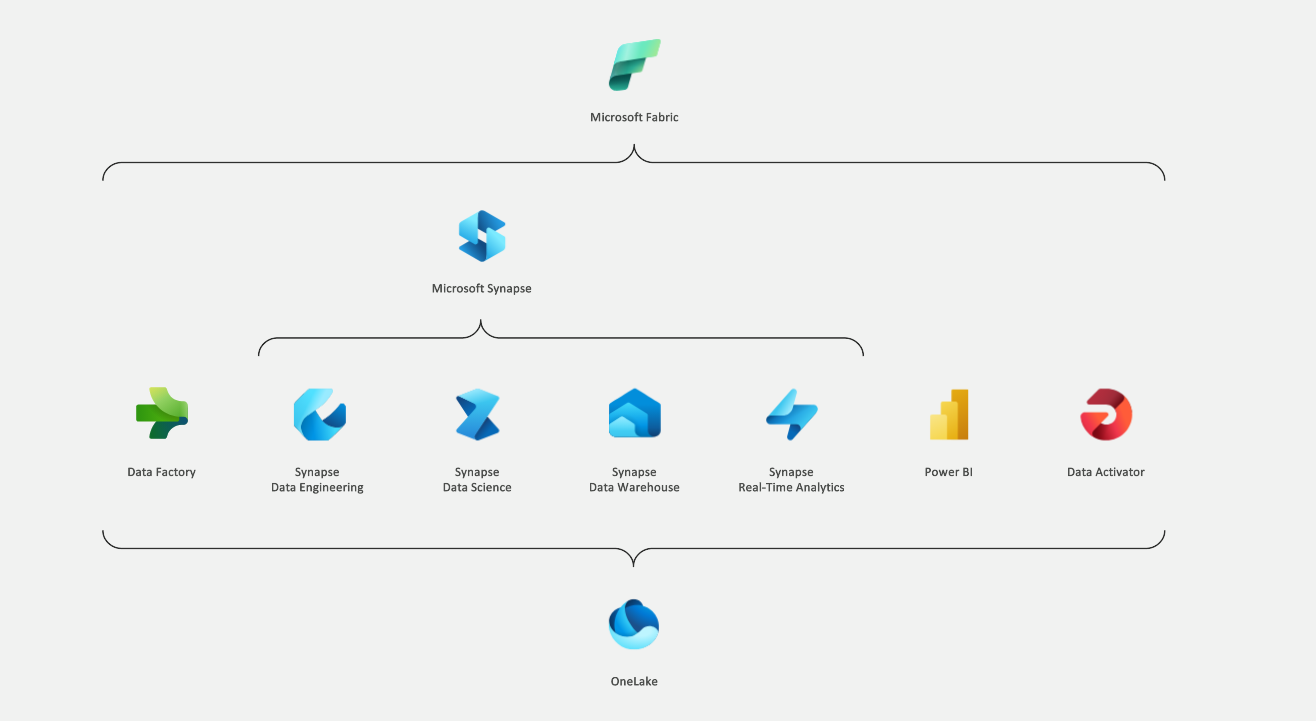
\includegraphics[width=1\textwidth]{./graphics/standvanzaken/fabric.png}
    \caption{Een overzicht van Microsoft Fabric~\autocite{Pykes2023}}
\end{figure}

Micrsoft Fabric is een platform dat verschillende Azure tools en services samen brengt. Het is een platform  dat zowel nieuwe als bestaande componenten van Power BI, Azure Synapse Analytics, Azure Data Factory en meer combineerd. Microsoft Fabric maakt gebruik van OneLake. Dit is een uniforme locatie voor het opslaan van organisatiegegevens, gebouwd op Azure Data Lake Storage Gen2~\autocite{Microsoft2024i}.

\subsection{Azure concepten en services}

De volgende onderdelen zijn belangrijk om te begrijpen. Het zijn concepten of Azure Services die worden gebruikt in de proof-of-concepts.

\subsubsection{Azure Resource Manager (ARM) templates}

Met behulp van Azure Resource Manager (ARM) templates kunnen resources beheert en geïmplementeerd worden met behulp van Infrastructure as Code (IaC). De template is een JSON bestand dat de infrastructuur en configuratie van een project definieert. Elke deployment van resources zal dus consistent zijn. Daarnaast zal Azure Resource Manager er voor zorgen dat resources in de juiste volgorde aangemaakt worden. Ook kunnen templates in verschillende bestanden ingedeeld worden zodat er bijvoorbeeld gebruik gemaakt kan worden van herbruikbare componenten. ARM templates kunnen geïntegreerd worden in CI/CD tools zodat release pipelines geautomatiseerd worden~\autocite{Azure2023}.

\subsubsection{Subscription}

Een Azure Subscription helpt bij het beheren van toegang tot Azure-services en bijhorende kosten. Binnen dit abonnement wordt de toegang tot resources beheerd en worden kosten bijgehouden. Elk abonnement wordt gekoppeld aan een factureringseenheid, zoals een creditcard of een zakelijke overeenkomst. Een Azure Subscription heeft vaak een gelaagde structuur. Deze bevat een aantal belangrijke elementen.\\

%\textbf{Resource Groups}

Ten eerste zijn er Resource Groups. Dit zijn logische containers waarin je vergelijkbare resources kunt plaatsen om het beheer te vereenvoudigen. Bijvoorbeeld, alle resources die nodig zijn voor een specifieke applicatie kunnen binnen één resourcegroep worden gegroepeerd~\autocite{Microsoft2024d}.

%\textbf{Roles en Role-Based Access Control (RBAC)}

Daarnaast zijn er Roles en en is er Role-Based Access Control (RBAC). Gebruikers en groepen kunnen rollen toegewezen krijgen die hun toegang tot resources binnen het abonnement bepalen. Deze rollen kunnen variëren van lezer tot eigenaar, afhankelijk van de benodigde toegangsrechten~\autocite{Microsoft2024e}.

%\textbf{Beleidsregels}

En ten slotte kunnen rganisaties beleidsregels instellen om te controleren welke resources kunnen worden gebruikt en hoe ze worden ingezet~\autocite{Microsoft2024f}.

\subsubsection{Data Lake}

Azure Data Lake is een cloudgebaseerde gegevensopslag ontworpen om bedrijven te helpen met het beheren en analyseren van grote hoeveelheden gestructureerde en ongestructureerde gegevens. De technologie achter Azure Data Lake bestaat uit drie hoofdelementen: Azure HDInsight, Azure Data Lake Storage en Azure Data Lake Analytics~\autocite{Awati2023a}.\\

HDInsight is een open source analytics platform voor het beheren van big data~\autocite{Awati2023a}.\\

Daarnaast is Data Lake Storage een veilige en schaalbare opslagservice die gegevens in hun oorspronkelijke formaat kan bewaren, ongeacht het type. Het is geoptimaliseerd voor big data-workloads, waardoor het grote hoeveelheden data van verschillende bronnen snel kan verwerken en opslaan~\autocite{Awati2023a}.\\

Aan de andere kant biedt Azure Data Lake Analytics een serverloze analyseomgeving waarin ontwikkelaars complexe queries kunnen uitvoeren op de opgeslagen gegevens. Door gebruik te maken van U-SQL, een querytaal die de kracht van SQL en C\# combineert, kunnen gebruikers gemakkelijk aangepaste analyses uitvoeren op grote datasets. Bovendien betaalt men alleen voor de verbruikte rekenkracht, waardoor dit model schaalbaar en kostenefficiënt is~\autocite{Awati2023a}.\\

Een belangrijk aspect van Azure Data Lake is dat kan integreren met andere Azure-services, zoals bijvoorbeeld Azure Synapse Analytics of Power BI.

\subsubsection{Key Vault}

Azure Key Vault maakt het mogelijk om veilig cryptografische sleutels en andere gevoelige informatie, zoals certificaten, API-sleutels en wachtwoorden op te slaan. De service biedt strenge toegangscontrole en encryptie om ervoor te zorgen dat gevoelige informatie privé en beschermd blijft. Met behulp van Azure Key Vault kunnen bijvoorbeeld secrets opgeslaan worden die dan via HTTPS toegankelijk zijn binnen beveiligde applicaties. Toegangsbeheer binnen Azure Key Vault wordt geregeld via Azure Active Directory (AAD), waardoor beheerders controle hebben over wie toegang heeft tot de Key Vault en wat ze kunnen doen met de opgeslagen geheimen. Bij het uitvoeren van ETL-processen (Extract, Transform, Load) is het van cruciaal belang dat gegevensbronnen en bestemmingen veilig met elkaar communiceren. Azure Key Vault speelt hierin een sleutelrol door als centrale opslagplaats voor alle gevoelige verbindingsinformatie te dienen, zoals database wachtwoorden en API-sleutels. Dit minimaliseert het risico op datalekken en verhoogt de veiligheid van het ETL-proces~\autocite{Microsoft2024g}.

\subsubsection{App Registration}

Met behulp van Azure App Registration kan een applicatie de nodige credentials krijgen tot Azure services en API's. Het is een soort paspoort voor een specifieke applicatie~\autocite{Anaparthy2023}.

\subsubsection{Cost Management}

In Azure is Micosoft Cost Management ontworpen voor het analyseren, monitoren en optimaliseren van kosten. Dankzij Cost Management kunnen rapporten en analyses gemaakt worden in de Azure Portal of in Power BI. Daarnaast kunnen er ook budgetten en waarschuwingen ingesteld worden. Ook zijn er verschillende hulpmiddelen beschikbaar die helpen bij het inschatten van cloudkosten. Kort samen gevat bevat het dus alle nodige tools voor het beheren, analyseren, inschatten en optimaliseren van kosten~\autocite{Microsoft2023}.

\section{Apache Spark}
\label{sec:apachespark}

Zowel Azure Data Factory, Azure Databricks en Azure Synapse Analytics maken gebruik van Apache Spark. Het is een gedistributeerd computing systeem dat het meest actieve Apache open source project is geworden. Het stelt zich in staat om data te verwerken in grote hoeveelheden met een relatief eenvoudig te gebruiken API voor zowel Python, Java, Scala en SQL. Daarnaast is het ook in staat om gegevenstransformaties en machine learning algoritmes te schrijven die relatief systeemonafhankelijk zijn~\autocite{Karau2017}.

\begin{figure}[H]
    \centering
    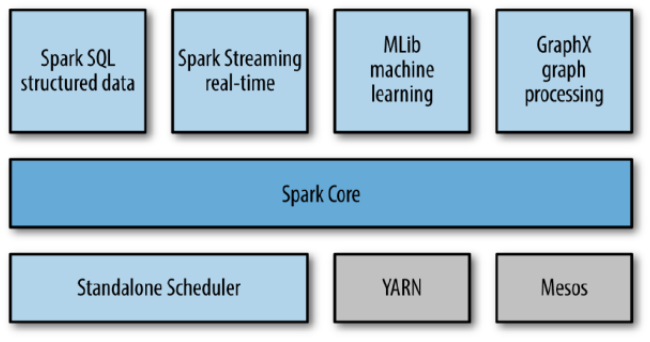
\includegraphics[width=1\textwidth]{./graphics/spark/spark-stack.png}
    \caption{Spark stack~\autocite{Karau2015}}
\end{figure}

Apache Spark is opgebouwd uit verschillende onderdelen. Als eerst hebben we Spark Core, dit is het fundament van Apache Spark en biedt de basisfunctionaliteit voor het verdelen en verwerken van gegevens in een gedistribueerde omgeving. Daarnaast hebben we Apache SQL, dit is een module voor het verwerken van gestructureerde gegevens met behulp van SQL-achtige queries. Spark Streaming aan de andere kant is een uitbreiding van de core Spark API die real-time gegevensverwerking mogelijk maakt. MLlib is dan weer de machine learning library van Apache Spark. GraphX is de bibliotheek binnen Apache Spark voor het verwerken van grafiekgegevens en het uitvoeren van grafiekanalyses. En ten slotte zijn er Cluster Managers, deze zijn verantwoordelijk voor het beheren van resources en het toewijzen van taken binnen een Spark-cluster. Voorbeelden hiervan zijn Apache Hadoop YARN, Apache Mesos en ingebouwde standalone-clustermodus van Spark~\autocite{Karau2015}.

%\section{Microsoft Azure}
%
%In de bachelorproef wordt er gebruikt gemaakt van meerdere Azure Services voor het implementeren van de proof-of-concepts. Hierdoor komen deze aan bod in de literatuurstudie om deze beter te begrijpen.\\
%
%Microsoft Azure is een cloud computing-platform dat door Microsoft wordt aangeboden. Het biedt een breed scala aan cloudgebaseerde oplossingen en services waarmee bedrijven en ontwikkelaars applicaties kunnen bouwen, implementeren en beheren. \\
%
%\begin{figure}[H]
%    \centering
%    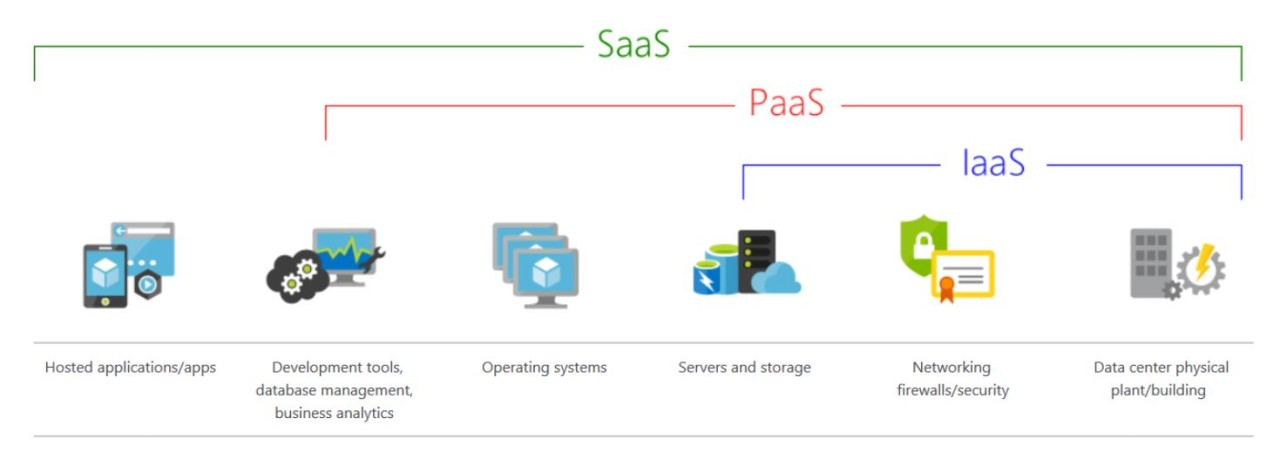
\includegraphics[width=1\textwidth]{./graphics/standvanzaken/verschillen.jpg}
%    \caption{Verschillen tussen IaaS, PaaS en SaaS~\autocite{Stoenescu2021}}
%\end{figure}
%
%Met Azure kunnen bedrijven gebruikmaken van Infrastructure as a Service (IaaS), waardoor ze onder andere virtuele machines, opslag en netwerken kunnen huren op basis van hun behoeften. Dit geeft organisaties de flexibiliteit om snel op te schalen zonder dat ze fysieke servers hoeven aan te schaffen. Daarnaast biedt het platform ook een Platform as a Service (PaaS), waarmee ontwikkelaars zich kunnen concentreren op het ontwikkelen van applicaties zonder zich zorgen te hoeven maken over de onderliggende infrastructuur. Ten slotte is er ook Software as a Service. Hierbij wordt er een applicatie gehost en beschikbaar gemaakt voor de gebruiker op basis van een subscription. Voorbeelden hier van zijn bijvorbeeld officetools (Microsoft Office 365)~\autocite{Suneetha2024}. \\
%
%Azure is sterk in dataopslag en -beheer, waarbij veilige en schaalbare opties worden aangeboden voor zowel gestructureerde als ongestructureerde gegevens. Bovendien kunnen organisaties gebruikmaken van analyse- en big data-services zoals Azure Synapse Analytics en HDInsight om inzichten te verkrijgen die strategische beslissingen ondersteunen~\autocite{Awati2023}. \\
%
%Darnaast biedt Azure ook encryptie, toegangsbeheer en compliance-certificeringen om gegevens veilig te houden~\autocite{Siddiqui2023}.

%\subsection{Microsoft Entra ID}
%
%Microsoft Entra ID, voorheen bekend als Azure Active Directory, is een uitgebreide cloud-gebaseerde identiteits- en toegangsbeheeroplossing van Microsoft. Het biedt organisaties de mogelijkheid om gebruikersidentiteiten effectief te beheren en toegang tot verschillende applicaties en diensten te controleren.
%
%Een van de kernfuncties van Entra ID is Single Sign-On (SSO), waarmee gebruikers met één enkele aanmelding toegang kunnen krijgen tot meerdere applicaties en diensten. Dit vereenvoudigt de gebruikerservaring en verhoogt de productiviteit, omdat herhaaldelijke inlogpogingen niet langer nodig zijn.
%

%\subsection{Azure Resource Manager (ARM) templates}
%
%Met behulp van Azure Resource Manager (ARM) templates kunnen resources beheert en geïmplementeerd worden met behulp van Infrastructure as Code (IaC). De template is een JSON bestand dat de infrastructuur en configuratie van een project definieert. Elke deployment van resources zal dus consistent zijn. Daarnaast zal Azure Resource Manager er voor zorgen dat resources in de juiste volgorde aangemaakt worden. Ook kunnen templates in verschillende bestanden ingedeeld worden zodat er bijvoorbeeld gebruik gemaakt kan worden van herbruikbare componenten. ARM templates kunnen geïntegreerd worden in CI/CD tools zodat release pipelines geautomatiseerd worden~\autocite{Azure2023}.
%
%\subsection{Subscription}
%
%Een Azure Subscription helpt bij het beheren van toegang tot Azure-services en bijhorende kosten. Binnen dit abonnement wordt de toegang tot resources beheerd en worden kosten bijgehouden. Elk abonnement wordt gekoppeld aan een factureringseenheid, zoals een creditcard of een zakelijke overeenkomst. Een Azure Subscription heeft vaak een gelaagde structuur. De belangrijkste elementen hiervan zijn:
%
%\subsubsection{Resource Groups}
%
%Dit zijn logische containers waarin je vergelijkbare resources kunt plaatsen om het beheer te vereenvoudigen. Bijvoorbeeld, alle resources die nodig zijn voor een specifieke applicatie kunnen binnen één resourcegroep worden gegroepeerd~\autocite{Microsoft2024d}.
%
%\subsubsection{Roles en Role-Based Access Control (RBAC)}
%
%Gebruikers en groepen kunnen rollen toegewezen krijgen die hun toegang tot resources binnen het abonnement bepalen. Deze rollen kunnen variëren van lezer tot eigenaar, afhankelijk van de benodigde toegangsrechten~\autocite{Microsoft2024e}.
%
%\subsubsection{Beleidsregels}
%
%Organisaties kunnen beleidsregels instellen om te controleren welke resources kunnen worden gebruikt en hoe ze worden ingezet~\autocite{Microsoft2024f}.
%
%\subsection{Data Lake}
%
%Azure Data Lake is een cloudgebaseerde gegevensopslag ontworpen om bedrijven te helpen met het beheren en analyseren van grote hoeveelheden gestructureerde en ongestructureerde gegevens. De technologie achter Azure Data Lake bestaat uit drie hoofdelementen: Azure HDInsight, Azure Data Lake Storage en Azure Data Lake Analytics~\autocite{Awati2023a}.\\
%
%HDInsight is een open source analytics platform voor het beheren van big data~\autocite{Awati2023a}.\\
%
%Daarnaast is Data Lake Storage een veilige en schaalbare opslagservice die gegevens in hun oorspronkelijke formaat kan bewaren, ongeacht het type. Het is geoptimaliseerd voor big data-workloads, waardoor het grote hoeveelheden data van verschillende bronnen snel kan verwerken en opslaan~\autocite{Awati2023a}.\\
%
%Aan de andere kant biedt Azure Data Lake Analytics een serverloze analyseomgeving waarin ontwikkelaars complexe queries kunnen uitvoeren op de opgeslagen gegevens. Door gebruik te maken van U-SQL, een querytaal die de kracht van SQL en C\# combineert, kunnen gebruikers gemakkelijk aangepaste analyses uitvoeren op grote datasets. Bovendien betaalt men alleen voor de verbruikte rekenkracht, waardoor dit model schaalbaar en kostenefficiënt is~\autocite{Awati2023a}.\\
%
%Een belangrijk aspect van Azure Data Lake is dat kan integreren met andere Azure-services, zoals bijvoorbeeld Azure Synapse Analytics of Power BI.
%
%\subsection{Key Vault}
%
%Azure Key Vault maakt het mogelijk om veilig cryptografische sleutels en andere gevoelige informatie, zoals certificaten, API-sleutels en wachtwoorden op te slaan. De service biedt strenge toegangscontrole en encryptie om ervoor te zorgen dat gevoelige informatie privé en beschermd blijft. Met behulp van Azure Key Vault kunnen bijvoorbeeld secrets opgeslaan worden die dan via HTTPS toegankelijk zijn binnen beveiligde applicaties. Toegangsbeheer binnen Azure Key Vault wordt geregeld via Azure Active Directory (AAD), waardoor beheerders controle hebben over wie toegang heeft tot de Key Vault en wat ze kunnen doen met de opgeslagen geheimen. Bij het uitvoeren van ETL-processen (Extract, Transform, Load) is het van cruciaal belang dat gegevensbronnen en bestemmingen veilig met elkaar communiceren. Azure Key Vault speelt hierin een sleutelrol door als centrale opslagplaats voor alle gevoelige verbindingsinformatie te dienen, zoals database wachtwoorden en API-sleutels. Dit minimaliseert het risico op datalekken en verhoogt de veiligheid van het ETL-proces~\autocite{Microsoft2024g}.
%
%\subsection{App Registration}
%
%Met behulp van Azure App Registration kan een applicatie de nodige credentials krijgen tot Azure services en API's. Het is een soort paspoort voor een specifieke applicatie~\autocite{Anaparthy2023}.
%
%\subsection{Cost Management}
%
%In Azure is Micosoft Cost Management ontworpen voor het analyseren, monitoren en optimaliseren van kosten. Dankzij Cost Management kunnen rapporten en analyses gemaakt worden in de Azure Portal of in Power BI. Daarnaast kunnen er ook budgetten en waarschuwingen ingesteld worden. Ook zijn er verschillende hulpmiddelen beschikbaar die helpen bij het inschatten van cloudkosten. Kort samen gevat bevat het dus alle nodige tools voor het beheren, analyseren, inschatten en optimaliseren van kosten~\autocite{Microsoft2023}.

%\section{Continuous Integration (CI) en Continuous Deployment (CD)}
%
%Bij Continuous Integration (CI) wordt de code van één of meerdere developers samen gevoegd, getest en gebouwd. Dit gebeurd continu. Een voorbeeld hiervan is dat een developer de code van zijn/haar GitHub branch merged op de ``main'' (of ``master'') branch van het project. Het doel van CI is dat deze ``main'' (of ``master'') branch gezond blijft en dat nieuwe aanpassingen door meerdere developers niet zorgt voor fouten in de code die resulteren in het falen van een build~\autocite{Jackson2020}.\\
%
%Continuous Delivery (CD) is een uitbereiding van Continuous Integration. Het is het automatiseren van het release process. Het zorgt er voor dat aanpassingen frequent gedeployed kunnen worden~\autocite{Jackson2020}.\\
%
%Ten slotte is er ook Continuous Deployment. Dit is een uitbereiding op Continuous Delivery en zorgt er voor dat code changes automatisch naar productie worden gepusht~\autocite{Jackson2020}.\\
%
%\section{Infrastructure as Code (IaC)}
%
%Infrastructure as Code (IaC) is een belangrijk concept in de wereld van moderne softwareontwikkeling. Het stelt teams in staat om infrastructuur te beheren met behulp van definitiebestanden, in plaats van fysieke hardwareconfiguratie of interactieve configuratietools. Deze bestanden helpen bij het automatiseren van het opzetten en onderhouden van infrastructuur, wat resulteert in snellere ontwikkelcycli en hogere betrouwbaarheid. Dit betekent dat de gehele infrastructuur, inclusief netwerken, virtuele machines en verbindingen, kan worden beheerd met scripts of declaraties. Het voordeel hiervan is dat er voor zowel de development en productie environment dezelfde infrastructuur opgezet kan worden. Het is dus snel en consistent. Doordat de definitiebestanden in IaC in source control opgeslaan kunnen worden, kunnen ook zo fouten makkelijker opgespoord worden~\autocite{Schults2024}.

%Als data engineer krijgt men data in veel verschillende vormen. Het is dus noodzakelijk omdeze data klaar te maken voor business analytics.
%
%Vandaag de dag bestaan er veel verschillende tools voor het implementeren van ETL's en ELT's. 
%
%\label{sec:toepassing-etl}
%
%\begin{itemize}
%    \item Azure Data Factory
%    \item AWS Glue
%    \item Google Cloud GPC Dataflow
%    
%\end{itemize}
%
%Dit hoofdstuk bevat je literatuurstudie. De inhoud gaat verder op de inleiding, maar zal het onderwerp van de bachelorproef *diepgaand* uitspitten. De bedoeling is dat de lezer na lezing van dit hoofdstuk helemaal op de hoogte is van de huidige stand van zaken (state-of-the-art) in het onderzoeksdomein. Iemand die niet vertrouwd is met het onderwerp, weet nu voldoende om de rest van het verhaal te kunnen volgen, zonder dat die er nog andere informatie moet over opzoeken \autocite{Pollefliet2011}.
%
%Je verwijst bij elke bewering die je doet, vakterm die je introduceert, enz.\ naar je bronnen. In \LaTeX{} kan dat met het commando \texttt{$\backslash${textcite\{\}}} of \texttt{$\backslash${autocite\{\}}}. Als argument van het commando geef je de ``sleutel'' van een ``record'' in een bibliografische databank in het Bib\LaTeX{}-formaat (een tekstbestand). Als je expliciet naar de auteur verwijst in de zin (narratieve referentie), gebruik je \texttt{$\backslash${}textcite\{\}}. Soms is de auteursnaam niet expliciet een onderdeel van de zin, dan gebruik je \texttt{$\backslash${}autocite\{\}} (referentie tussen haakjes). Dit gebruik je bv.~bij een citaat, of om in het bijschrift van een overgenomen afbeelding, broncode, tabel, enz. te verwijzen naar de bron. In de volgende paragraaf een voorbeeld van elk.
%
%\textcite{Knuth1998} schreef een van de standaardwerken over sorteer- en zoekalgoritmen. Experten zijn het erover eens dat cloud computing een interessante opportuniteit vormen, zowel voor gebruikers als voor dienstverleners op vlak van informatietechnologie~\autocite{Creeger2009}.
%
%Let er ook op: het \texttt{cite}-commando voor de punt, dus binnen de zin. Je verwijst meteen naar een bron in de eerste zin die erop gebaseerd is, dus niet pas op het einde van een paragraaf.
%
%\lipsum[7-20]
